\documentclass[11pt]{article}
\usepackage[letterpaper,top=.62in,bottom=.64in,left=.70in,right=.70in,headheight=15pt,footskip=.28in]{geometry}
\usepackage[T1]{fontenc}
\usepackage{lmodern}
\usepackage{microtype}
\usepackage{graphicx}
\usepackage{booktabs}
\usepackage{tabularx}
\usepackage{longtable}
\usepackage{array}
\usepackage{amsmath}
\usepackage{xcolor}
\usepackage{caption}
\usepackage{float}
\usepackage{needspace}
\usepackage{fancyhdr}
\usepackage{titlesec}

\definecolor{rulegray}{HTML}{68717A}
\definecolor{boxfill}{HTML}{F3F6F8}
\newcolumntype{Y}{>{\raggedright\arraybackslash}X}
\newcolumntype{C}{>{\centering\arraybackslash}X}
\renewcommand{\thesection}{S\arabic{section}}
\renewcommand{\thefigure}{S\arabic{figure}}
\titleformat{\section}{\large\bfseries}{\thesection}{.55em}{}
\titlespacing*{\section}{0pt}{9pt plus 2pt minus 1pt}{4pt}
\setlength{\parindent}{0pt}
\setlength{\parskip}{3.2pt plus .5pt}
\setlength{\textfloatsep}{7pt plus 2pt minus 2pt}
\setlength{\floatsep}{6pt plus 2pt minus 2pt}
\setlength{\intextsep}{6pt plus 2pt minus 2pt}
\renewcommand{\arraystretch}{1.10}
\setlength{\tabcolsep}{3.4pt}
\newcommand{\tablefont}{\fontsize{9.5}{11.2}\selectfont}
\newcommand{\sourcecaption}[1]{\Needspace{10\baselineskip}\vspace{2pt}{\small\bfseries #1}\par\vspace{2pt}}
\captionsetup{font=small,labelfont=bf,labelsep=period,justification=raggedright,singlelinecheck=false,skip=3pt}
\widowpenalty=10000
\clubpenalty=10000
\displaywidowpenalty=10000
\hbadness=10000
\pagestyle{fancy}
\fancyhf{}
\lhead{\small Supplementary Material}
\rhead{\small Molecular specificity from electrophysiology}
\cfoot{\small S\arabic{page}}

\begin{document}
\begin{center}
{\Large\bfseries Supplementary Material}\par\vspace{3pt}
{\large Testing Molecular Specificity in Electrophysiology-to-Transcript Prediction\\with Matched Negative Controls}\par\vspace{5pt}
{\normalsize ICCKE 2026}\par
\end{center}
\vspace{-2pt}
\colorbox{boxfill}{\parbox{.965\linewidth}{\small
\textbf{Scope.} This supplement reports the complete donor-grouped out-of-fold results and the validated primary and sensitivity analyses supporting the main text. Tables S1--S50 are provided as machine-readable CSV files and Figures S1--S5 in publication-ready formats. All entries are taken directly from validated analysis outputs; no model was refitted and no numerical result was recalculated. Complete CSV tables are supplied where only a concise display is possible within the page limit.}}

\section{Data Sources and Cohort Construction}
Cells were joined one-to-one by \texttt{cell\_specimen\_id}. The fixed analytic cohort contains 3,410 mouse visual-cortex inhibitory neurons from 871 donor groups and 6 broad subclasses. Tables S1--S3 provide the cohort characteristics, donor counts, and canonical crosswalk. Donor identity defined every outer split. Raw Allen data are not redistributed.

\sourcecaption{Cohort composition, donor counts, and cell-level crosswalk (Tables S1--S3).}
\begin{center}\tablefont
\begin{tabular}{lr}
\toprule
Item & Value \\
\midrule
Paired MAT cells before public-metadata matching & 3,411 \\
Unmatched specimen excluded & 1 \\
Cells in analytic cohort & 3,410 \\
Donor groups & 871 \\
Broad subclasses & 6 \\
Outer donor-disjoint folds & 3 (1,137 / 1,136 / 1,137 cells) \\
Canonical cell-crosswalk rows & 3,410 \\
Modeled electrophysiology predictors & 23 \\
\bottomrule
\end{tabular}
\end{center}

\section{Electrophysiology Predictors}
The source matrix contained 24 variables. Modeling retained \texttt{rheobase\_\allowbreak{}i} and removed its exact duplicate, \texttt{stimulus\_\allowbreak{}amplitude\_\allowbreak{}0\_\allowbreak{}long\_\allowbreak{}square}, leaving 23 nonredundant IPFX predictors; 44 waveform principal components were excluded. Release-level standardization and clipping at $\pm6$ SD occurred upstream. Physical-unit inversion from the saved affine transform is approximate, and observations at the clipping boundaries remain censored. Only downstream median imputation and model-specific scaling were fitted within each outer-training fold.

\sourcecaption{Electrophysiological predictors used in the 23-feature analysis (Table S4).}
\begin{center}\fontsize{9}{10.1}\selectfont
\renewcommand{\arraystretch}{1.00}
\begin{tabularx}{\linewidth}{@{}rYlrYl@{}}
\toprule
No. & Exact feature key & Unit & No. & Exact feature key & Unit \\
\midrule
1 & \texttt{ap\_\allowbreak{}1\_\allowbreak{}threshold\_\allowbreak{}v\_\allowbreak{}short\_\allowbreak{}square} & mV & 13 & \texttt{sag\_\allowbreak{}measured\_\allowbreak{}at} & mV \\
2 & \texttt{ap\_\allowbreak{}1\_\allowbreak{}peak\_\allowbreak{}v\_\allowbreak{}short\_\allowbreak{}square} & mV & 14 & \texttt{rheobase\_\allowbreak{}i} & pA \\
3 & \texttt{ap\_\allowbreak{}1\_\allowbreak{}upstroke\_\allowbreak{}short\_\allowbreak{}square} & V/s (equivalent mV/ms) & 15 & \texttt{ap\_\allowbreak{}1\_\allowbreak{}threshold\_\allowbreak{}v\_\allowbreak{}0\_\allowbreak{}long\_\allowbreak{}square} & mV \\
4 & \texttt{ap\_\allowbreak{}1\_\allowbreak{}downstroke\_\allowbreak{}short\_\allowbreak{}square} & V/s (equivalent mV/ms) & 16 & \texttt{ap\_\allowbreak{}1\_\allowbreak{}peak\_\allowbreak{}v\_\allowbreak{}0\_\allowbreak{}long\_\allowbreak{}square} & mV \\
5 & \texttt{ap\_\allowbreak{}1\_\allowbreak{}upstroke\_\allowbreak{}downstroke\_\allowbreak{}ratio\_\allowbreak{}short\_\allowbreak{}square} & dimensionless & 17 & \texttt{ap\_\allowbreak{}1\_\allowbreak{}upstroke\_\allowbreak{}0\_\allowbreak{}long\_\allowbreak{}square} & V/s (equivalent mV/ms) \\
6 & \texttt{ap\_\allowbreak{}1\_\allowbreak{}width\_\allowbreak{}short\_\allowbreak{}square} & s & 18 & \texttt{ap\_\allowbreak{}1\_\allowbreak{}downstroke\_\allowbreak{}0\_\allowbreak{}long\_\allowbreak{}square} & V/s (equivalent mV/ms) \\
7 & \texttt{ap\_\allowbreak{}1\_\allowbreak{}fast\_\allowbreak{}trough\_\allowbreak{}v\_\allowbreak{}short\_\allowbreak{}square} & mV & 19 & \texttt{ap\_\allowbreak{}1\_\allowbreak{}upstroke\_\allowbreak{}downstroke\_\allowbreak{}ratio\_\allowbreak{}0\_\allowbreak{}long\_\allowbreak{}square} & dimensionless \\
8 & \texttt{short\_\allowbreak{}square\_\allowbreak{}current} & pA & 20 & \texttt{ap\_\allowbreak{}1\_\allowbreak{}width\_\allowbreak{}0\_\allowbreak{}long\_\allowbreak{}square} & s \\
9 & \texttt{input\_\allowbreak{}resistance} & M$\Omega$ & 21 & \texttt{ap\_\allowbreak{}1\_\allowbreak{}fast\_\allowbreak{}trough\_\allowbreak{}v\_\allowbreak{}0\_\allowbreak{}long\_\allowbreak{}square} & mV \\
10 & \texttt{tau} & s & 22 & \texttt{avg\_\allowbreak{}rate\_\allowbreak{}0\_\allowbreak{}long\_\allowbreak{}square} & Hz \\
11 & \texttt{v\_\allowbreak{}baseline} & mV & 23 & \texttt{latency\_\allowbreak{}0\_\allowbreak{}long\_\allowbreak{}square} & s \\
12 & \texttt{sag\_\allowbreak{}nearest\_\allowbreak{}minus\_\allowbreak{}100} & dimensionless &  & &  \\
\bottomrule
\end{tabularx}
\end{center}

\section{Molecular Module Definitions}
Targets were unweighted means of $\log_2(\mathrm{CPM}+1)$ across 6 prespecified gene modules; CPM denominators used all 45,768 count rows. Exact-symbol coverage was 95/96. Exact \texttt{Scn2a} was absent and was not replaced by \texttt{Scn2a1}; the primary NaV score therefore contains 6 observed genes. NaV7 is reported only as a separate sensitivity.

\sourcecaption{Gene-module definitions and exact-symbol coverage (Tables S5--S6).}
\begin{center}\tablefont
\begin{tabularx}{\linewidth}{@{}lcYl@{}}
\toprule
Module & Used/requested & Genes used & Missing exact symbol \\
\midrule
NaV & 6/7 & Scn1a, Scn3a, Scn8a, Scn9a, Scn10a, Scn11a & Scn2a \\
Kv & 40/40 & Kcna1, Kcna2, Kcna3, Kcna4, Kcna5, Kcna6, Kcna7, Kcna10, Kcnb1, Kcnb2, Kcnc1, Kcnc2, Kcnc3, Kcnc4, Kcnd1, Kcnd2, Kcnd3, Kcnf1, Kcng1, Kcng2, Kcng3, Kcng4, Kcnq1, Kcnq2, Kcnq3, Kcnq4, Kcnq5, Kcns1, Kcns2, Kcns3, Kcnv1, Kcnv2, Kcnh1, Kcnh2, Kcnh3, Kcnh4, Kcnh5, Kcnh6, Kcnh7, Kcnh8 & -- \\
CaV & 10/10 & Cacna1s, Cacna1c, Cacna1d, Cacna1f, Cacna1a, Cacna1b, Cacna1e, Cacna1g, Cacna1h, Cacna1i & -- \\
HCN & 4/4 & Hcn1, Hcn2, Hcn3, Hcn4 & -- \\
GABAA & 19/19 & Gabra1, Gabra2, Gabra3, Gabra4, Gabra5, Gabra6, Gabrb1, Gabrb2, Gabrb3, Gabrg1, Gabrg2, Gabrg3, Gabrd, Gabre, Gabrp, Gabrq, Gabrr1, Gabrr2, Gabrr3 & -- \\
iGluR & 16/16 & Gria1, Gria2, Gria3, Gria4, Grik1, Grik2, Grik3, Grik4, Grik5, Grin1, Grin2a, Grin2b, Grin2c, Grin2d, Grin3a, Grin3b & -- \\
\bottomrule
\end{tabularx}
\end{center}

\section{Model Specifications}
Elastic Net, XGBoost, and a small multilayer perceptron (MLP) were evaluated on the same donor-disjoint outer folds. Candidate selection used one 20\% donor-disjoint inner split within each outer-training set. Tables S7--S9 provide the fixed search spaces, MLP training and early-stopping procedure, and every fold-specific selected setting.

\sourcecaption{Model search spaces, training procedures, and selected hyperparameters (Tables S7--S9).}
\begin{center}\tablefont
\setlength{\tabcolsep}{3pt}
\begin{tabularx}{\linewidth}{@{}p{.105\linewidth}p{.37\linewidth}Y@{}}
\toprule
Model & Candidate-specific values & Training and preprocessing procedure \\
\midrule
Elastic Net & $\alpha\in\{.001, .010, .100, 1.000\}$, $\ell_1$ ratio $\in\{.1, .5, .9\}$ (12 candidates) & Maximum 5,000 iterations; seed 42; fold-local median imputation and standardization. \\
XGBoost & (250/2/.05/1); (400/2/.03/3); (250/3/.05/3); (300/4/.03/5) (trees/depth/rate/$L_2$) & Subsample .8; column sample .8; min-child weight 1; $L_1=0$; gamma 0; objective \texttt{reg:squarederror}; tree method \texttt{hist}; 1 job; seed 42; fold-local median imputation. \\
MLP & Hidden layers 64/32; activation relu; solver adam; $L_2=.001$; \texttt{learning\_\allowbreak{}rate}=\texttt{constant}; \texttt{learning\_\allowbreak{}rate\_\allowbreak{}init}=.001; \texttt{batch\_\allowbreak{}size}=\texttt{auto}; \texttt{shuffle}=True; seeds 42/123/2026 & \texttt{inner\_\allowbreak{}split\_\allowbreak{}method}=\texttt{GroupShuffleSplit}; \texttt{inner\_\allowbreak{}validation\_\allowbreak{}fraction}=.2; \texttt{inner\_\allowbreak{}validation\_\allowbreak{}grouped}=True; \texttt{early\_\allowbreak{}stopping}=\texttt{group\_\allowbreak{}aware\_\allowbreak{}manual}; \texttt{sklearn\_\allowbreak{}early\_\allowbreak{}stopping}=False; estimator validation fraction 0.15 is inert. Maximum 300 epochs; patience 20; $\mathrm{min\_delta}=1e-05$; epoch selected by minimum validation RMSE; fresh full outer-train refit; \texttt{n\_\allowbreak{}iter\_\allowbreak{}}=\texttt{selected\_\allowbreak{}epoch} for every saved model. \\
\bottomrule
\end{tabularx}
\end{center}

\section{Complete Primary Performance}
Pooled donor-grouped OOF $R^2$ was the primary predictive metric. Table S10 reports every model--module combination with $R^2$, MAE, RMSE, and Spearman $\rho$; Table S11 gives the corresponding fold-level results. Individual-model confidence intervals are available only for the 24-feature reference analysis (Table S12) and are not presented for the 23-feature analysis. Table S13 gives the direct 23-feature-versus-24-feature sensitivity.

{\tablefont
\sourcecaption{Complete pooled OOF performance for the 23-feature analysis (Table S10; $n=3,410$).}
\begin{longtable}{@{}llrrrr@{}}
\toprule
Module & Model & $R^2$ & MAE & RMSE & Spearman $\rho$ \\
\midrule
\endfirsthead
\multicolumn{6}{l}{\small\itshape Table S10 continued}\\[2pt]
\toprule
Module & Model & $R^2$ & MAE & RMSE & Spearman $\rho$ \\
\midrule
\endhead
NaV & Dummy & -.003 & .670 & .876 & -.043 \\
NaV & Elastic Net & .121 & .633 & .820 & .355 \\
NaV & XGBoost & .133 & .626 & .814 & .380 \\
NaV & MLP & .082 & .646 & .838 & .346 \\
NaV & Subclass Ridge & .102 & .633 & .829 & .300 \\
NaV & Ephys + subclass Ridge & .136 & .626 & .813 & .388 \\
Kv & Dummy & -.002 & .423 & .553 & -.041 \\
Kv & Elastic Net & .046 & .413 & .539 & .221 \\
Kv & XGBoost & .046 & .410 & .539 & .226 \\
Kv & MLP & -.015 & .426 & .556 & .219 \\
Kv & Subclass Ridge & .042 & .413 & .541 & .179 \\
Kv & Ephys + subclass Ridge & .065 & .408 & .534 & .262 \\
CaV & Dummy & -.002 & .734 & .965 & -.035 \\
CaV & Elastic Net & .094 & .674 & .918 & .361 \\
CaV & XGBoost & .106 & .663 & .912 & .395 \\
CaV & MLP & .035 & .696 & .947 & .342 \\
CaV & Subclass Ridge & .104 & .664 & .913 & .351 \\
CaV & Ephys + subclass Ridge & .114 & .662 & .908 & .399 \\
HCN & Dummy & -.001 & .932 & 1.172 & -.023 \\
HCN & Elastic Net & .064 & .904 & 1.133 & .256 \\
HCN & XGBoost & .057 & .906 & 1.138 & .248 \\
HCN & MLP & .011 & .926 & 1.165 & .221 \\
HCN & Subclass Ridge & .041 & .910 & 1.147 & .171 \\
HCN & Ephys + subclass Ridge & .057 & .907 & 1.138 & .248 \\
GABAA & Dummy & -.001 & .634 & .794 & -.032 \\
GABAA & Elastic Net & .260 & .526 & .682 & .528 \\
GABAA & XGBoost & .329 & .494 & .650 & .574 \\
GABAA & MLP & .314 & .501 & .657 & .567 \\
GABAA & Subclass Ridge & .177 & .551 & .720 & .391 \\
GABAA & Ephys + subclass Ridge & .319 & .499 & .655 & .574 \\
iGluR & Dummy & -.002 & .765 & 1.000 & -.019 \\
iGluR & Elastic Net & .258 & .612 & .861 & .602 \\
iGluR & XGBoost & .295 & .581 & .840 & .631 \\
iGluR & MLP & .206 & .622 & .891 & .582 \\
iGluR & Subclass Ridge & .327 & .560 & .820 & .637 \\
iGluR & Ephys + subclass Ridge & .340 & .557 & .812 & .667 \\
\bottomrule
\end{longtable}}

\sourcecaption{Change in $R^2$: 23-feature minus 24-feature reference analysis (Table S13).}
\begin{center}\tablefont
\begin{tabular}{lrrr}
\toprule
Module & Elastic Net & XGBoost & MLP \\
\midrule
NaV & -.000096 & .003851 & -.010114 \\
Kv & -.000003 & -.003146 & -.019469 \\
CaV & .000081 & .000306 & -.013158 \\
HCN & -.000005 & -.003854 & .000731 \\
GABAA & .000001 & -.000816 & -.011799 \\
iGluR & -.000013 & .000682 & -.019147 \\
\bottomrule
\end{tabular}
\end{center}

\section{Formal Model Comparisons}
The prespecified contrasts used 5,000 paired donor-cluster bootstrap draws. Positive $\Delta R^2$ favors the first model named. Table S14 contains the complete metric-specific comparisons; Table S15 gives the prespecified $R^2$ family with Benjamini--Hochberg adjustment. Corrected positive support for XGBoost over Elastic Net was confined to GABAA and iGluR. Positive values favor the first model; a negative BH-resolved contrast indicates that the first model performed worse.

\sourcecaption{Paired donor-cluster bootstrap comparisons for pooled OOF $R^2$ (Table S15).}
\begin{center}\tablefont
\begin{tabular}{llrrrr}
\toprule
Module & Contrast & $\Delta R^2$ & 95\% CI & BH $q$ & BH-resolved \\
\midrule
NaV & XGB - EN & .013 & [-.001, .026] & .0825 & no \\
NaV & MLP - EN & -.038 & [-.061, -.017] & .0011 & yes \\
NaV & MLP - XGB & -.051 & [-.071, -.032] & .0006 & yes \\
Kv & XGB - EN & -.0001 & [-.015, .015] & .9942 & no \\
Kv & MLP - EN & -.061 & [-.090, -.033] & .0006 & yes \\
Kv & MLP - XGB & -.061 & [-.087, -.037] & .0006 & yes \\
CaV & XGB - EN & .012 & [-.001, .025] & .0825 & no \\
CaV & MLP - EN & -.059 & [-.084, -.035] & .0006 & yes \\
CaV & MLP - XGB & -.071 & [-.095, -.048] & .0006 & yes \\
HCN & XGB - EN & -.007 & [-.018, .004] & .2189 & no \\
HCN & MLP - EN & -.053 & [-.073, -.033] & .0006 & yes \\
HCN & MLP - XGB & -.046 & [-.066, -.027] & .0006 & yes \\
GABAA & XGB - EN & .069 & [.052, .086] & .0006 & yes \\
GABAA & MLP - EN & .054 & [.030, .077] & .0006 & yes \\
GABAA & MLP - XGB & -.015 & [-.037, .006] & .1818 & no \\
iGluR & XGB - EN & .036 & [.021, .053] & .0006 & yes \\
iGluR & MLP - EN & -.052 & [-.079, -.028] & .0006 & yes \\
iGluR & MLP - XGB & -.088 & [-.117, -.064] & .0006 & yes \\
\bottomrule
\end{tabular}
\end{center}

\section{Permutation Diagnostics}
Both permutation families were applied to saved OOF predictions without model refitting; they are association diagnostics rather than algorithm-level randomization tests. The cell-level family permuted truth within subclass. The donor-level family permuted subclass-adjusted donor truth summaries across 871 donors.

\sourcecaption{Permutation diagnostics based on saved OOF predictions, without model refitting (Table S16; 5,000 permutations).}
\begin{center}\tablefont
\begin{tabular}{llrrrr}
\toprule
Module & Model & Cell Spearman $\rho$ & Cell $p$ & Donor adjusted Spearman $\rho$ & Donor $p$ \\
\midrule
NaV & Elastic Net & .355 & .0002 & .241 & .0002 \\
NaV & XGBoost & .380 & .0002 & .238 & .0002 \\
NaV & MLP & .346 & .0002 & .245 & .0002 \\
Kv & Elastic Net & .221 & .0002 & .138 & .0004 \\
Kv & XGBoost & .226 & .0002 & .180 & .0002 \\
Kv & MLP & .219 & .0002 & .192 & .0002 \\
CaV & Elastic Net & .361 & .0002 & .092 & .0066 \\
CaV & XGBoost & .395 & .0002 & .133 & .0002 \\
CaV & MLP & .342 & .0002 & .142 & .0002 \\
HCN & Elastic Net & .256 & .0002 & .101 & .0040 \\
HCN & XGBoost & .248 & .0002 & .116 & .0004 \\
HCN & MLP & .221 & .0002 & .151 & .0002 \\
GABAA & Elastic Net & .528 & .0002 & .329 & .0002 \\
GABAA & XGBoost & .574 & .0002 & .380 & .0002 \\
GABAA & MLP & .567 & .0002 & .386 & .0002 \\
iGluR & Elastic Net & .602 & .0002 & .143 & .0004 \\
iGluR & XGBoost & .631 & .0002 & .215 & .0002 \\
iGluR & MLP & .582 & .0002 & .204 & .0002 \\
\bottomrule
\end{tabular}
\end{center}

\section{Matched Negative Controls}
Each observed module was compared with 1,000 same-size gene sets matched on gene-level mean $\log_2(\mathrm{CPM}+1)$ and detection rate; matching did not directly use co-expression or within-module coherence. These two quantities were standardized over eligible non-module genes. For each target gene, up to 128 nearest candidates were ordered by standardized Euclidean distance and selected without replacement; all primary-module genes were excluded. A set was accepted only when maximum and mean per-gene distances were at most .50 and .25, respectively, and absolute module-level expression and detection imbalances were at most .10 and .10; up to 200 deterministic proposals were allowed. The observed-module XGBoost configuration was reused without control-outcome tuning. All 6,000 sets met these criteria. The percentile is $100\,\Pr(R^2_{control}\le R^2_{observed})$ and the empirical $p$ value is $(1+\#\{R^2_{control}\ge R^2_{observed}\})/(B+1)$.

\sourcecaption{Primary matched-control specificity analysis on unadjusted module scores (Table S18; separate 6-test family).}
\begin{center}\tablefont
\begin{tabular}{lrrrrrrl}
\toprule
Module & Observed $R^2$ & Null median & Null P95 & Percentile & $p$ & BH $q$ & BH-supported \\
\midrule
NaV & .133 & .029 & .131 & 95.1 & .0500 & .0999 & no \\
Kv & .046 & .101 & .185 & 10.1 & .8991 & .8991 & no \\
CaV & .106 & .056 & .163 & 80.5 & .1958 & .2937 & no \\
HCN & .057 & .023 & .123 & 74.2 & .2587 & .3105 & no \\
GABAA & .329 & .071 & .200 & 99.8 & .0030 & .0180 & yes \\
iGluR & .295 & .084 & .230 & 98.7 & .0140 & .0420 & yes \\
\bottomrule
\end{tabular}
\end{center}

\sourcecaption{Matching diagnostics and fixed-versus-retuned sensitivity (Tables S19 and S21). Retuning used 50 controls per module; $\Delta R^2$ is retuned minus fixed.}
\begin{center}\tablefont
\setlength{\tabcolsep}{2.7pt}
\begin{tabular}{lrrrrrrr}
\toprule
Module & Passed & Mean dist. & Max dist. & Max $|\Delta z_E|$ & Max $|\Delta z_D|$ & \shortstack{Rejected\\proposals} & Median $\Delta R^2$ \\
\midrule
NaV & 1,000/1,000 & .043 & .174 & .052 & .042 & 0 & .0007 \\
Kv & 1,000/1,000 & .072 & .328 & .032 & .038 & 0 & .0034 \\
CaV & 1,000/1,000 & .068 & .211 & .058 & .057 & 0 & .0016 \\
HCN & 1,000/1,000 & .071 & .169 & .081 & .082 & 0 & .0038 \\
GABAA & 1,000/1,000 & .070 & .271 & .047 & .068 & 0 & .0079 \\
iGluR & 1,000/1,000 & .156 & .497 & .099 & .082 & 56,007 & .0039 \\
\bottomrule
\end{tabular}
\end{center}
{\small \textit{Note.} Rejected proposals are unsuccessful deterministic candidate-set proposals generated before obtaining the 1,000 accepted matched sets; they are not excluded cells or failed final controls.}

\begin{figure}[H]
\centering
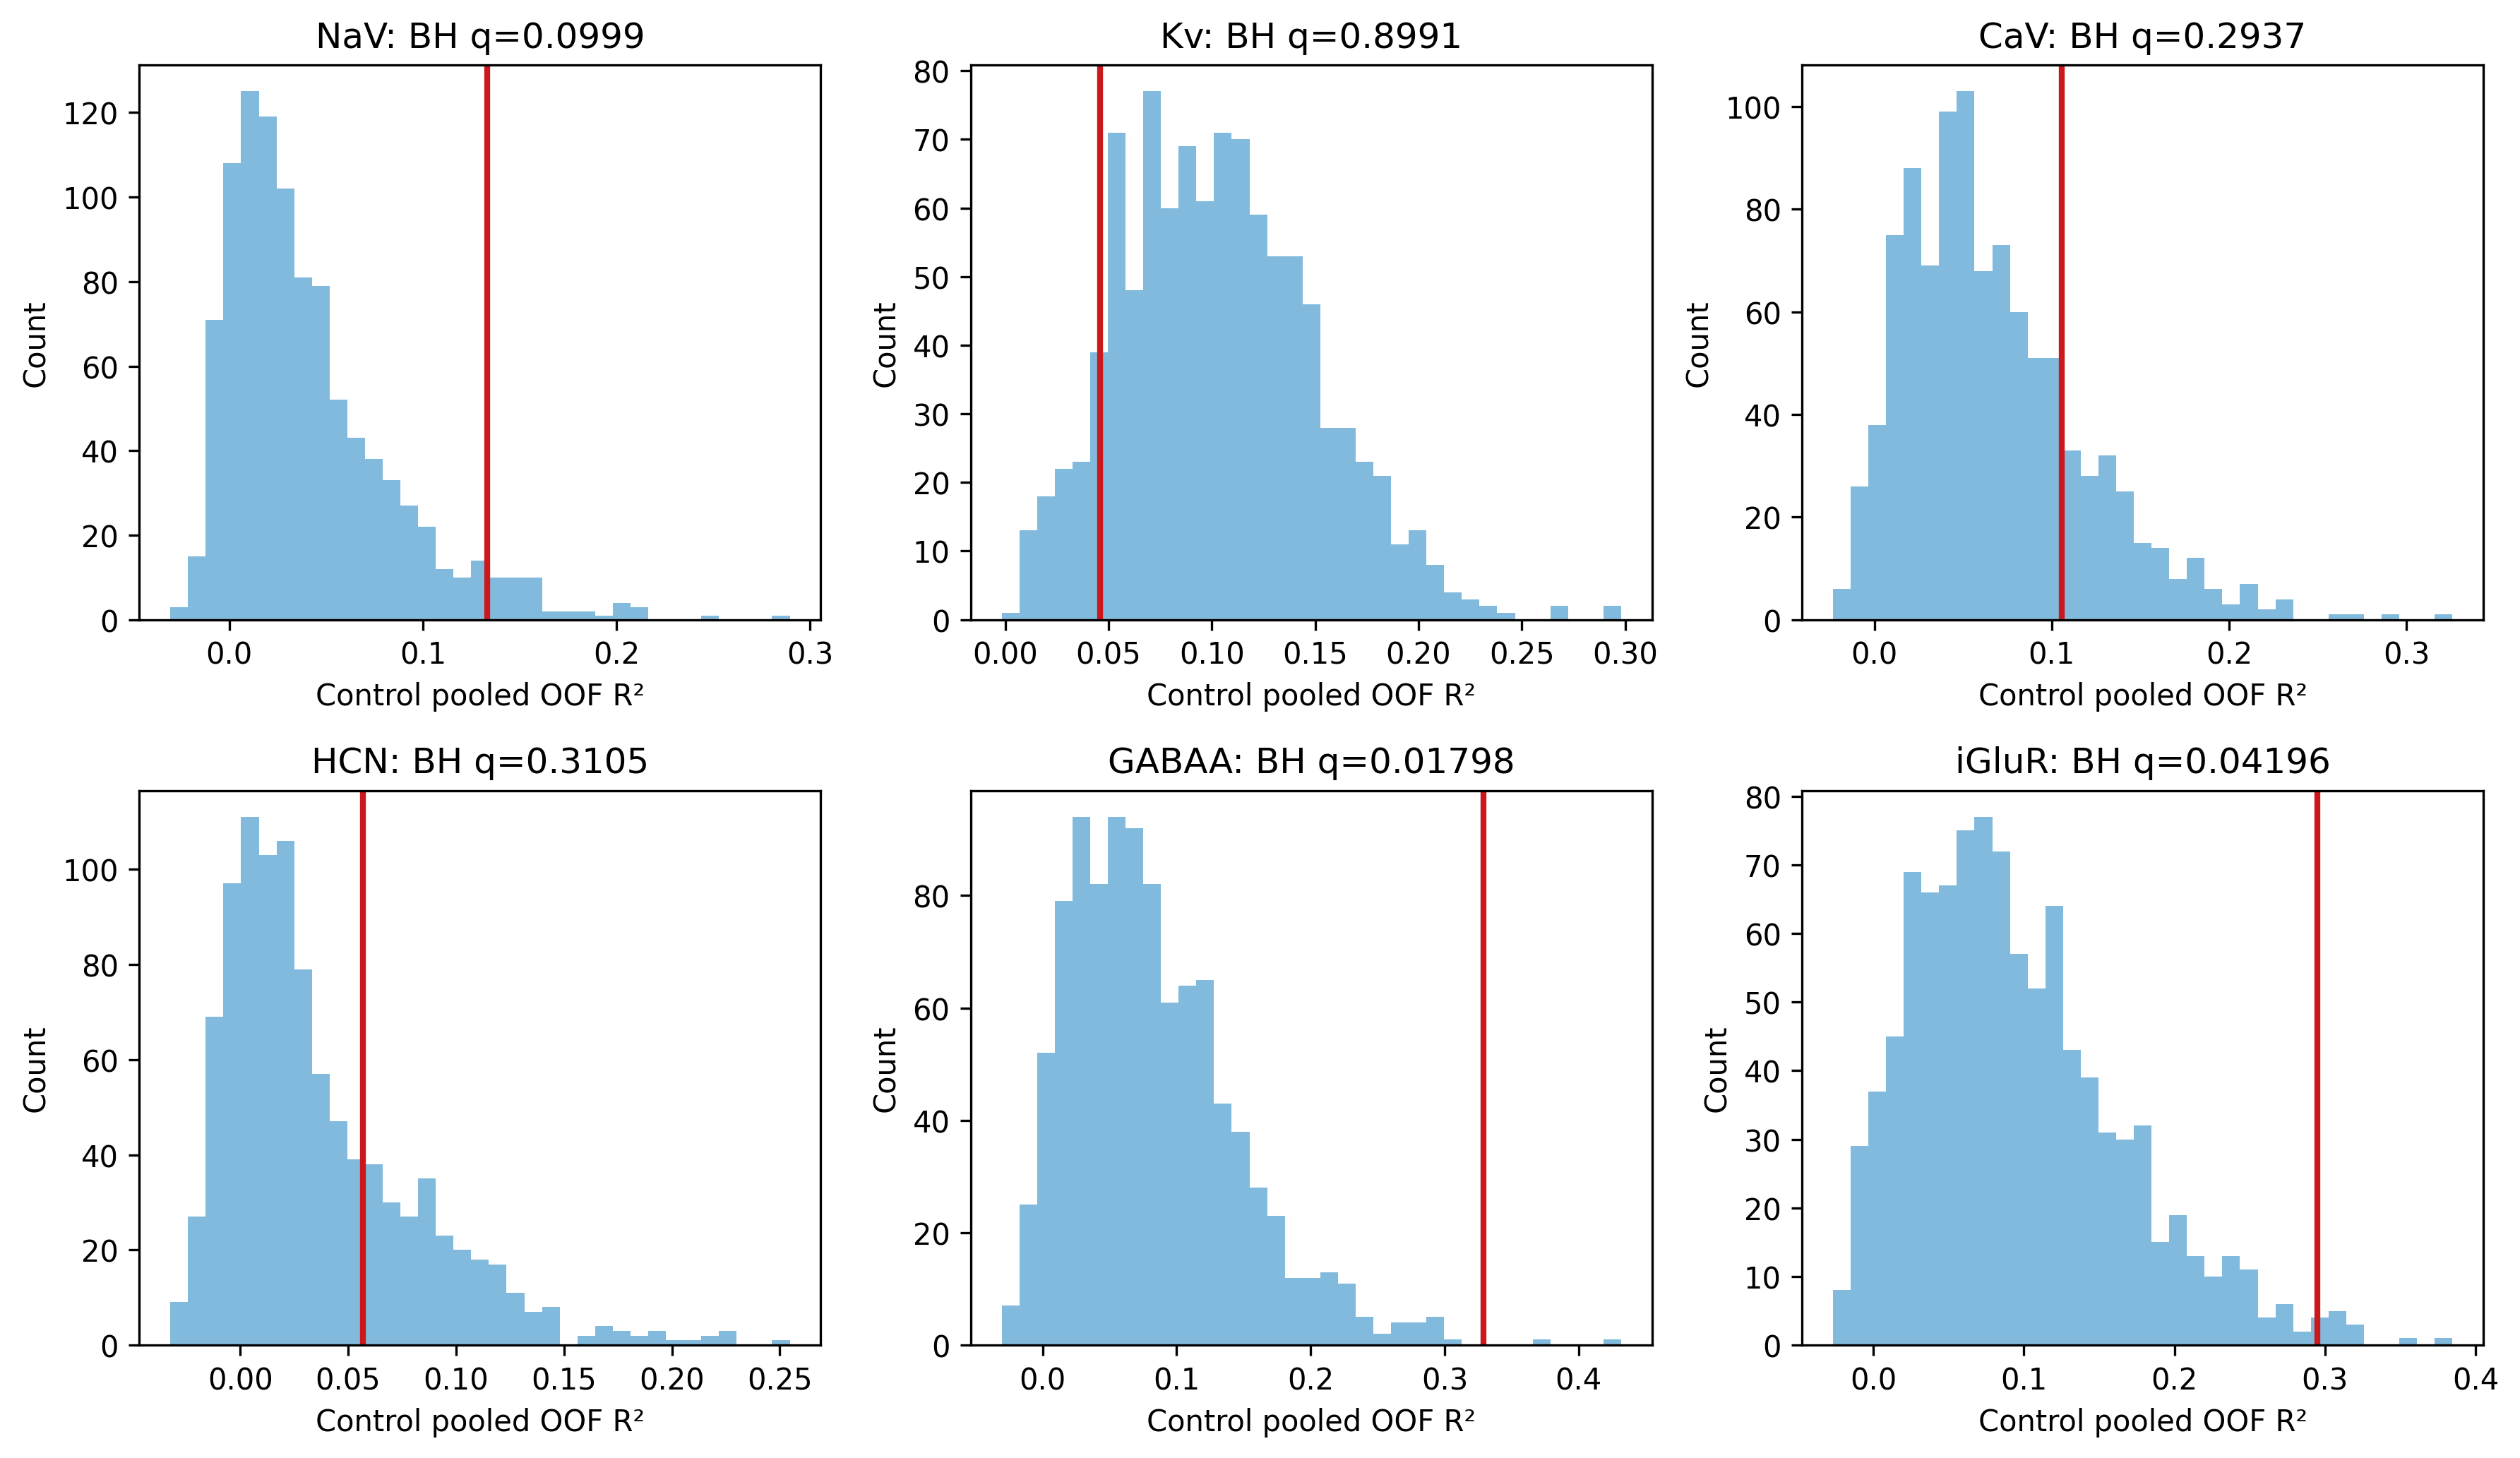
\includegraphics[width=.95\linewidth]{figures/Figure_S01_matched_negative_controls.png}
\caption{Matched negative-control specificity. The primary raw family is kept separate from the technical-residualized sensitivity family.}
\label{fig:controls}
\end{figure}

\section{Technical Targets and Residualized Specificity}
Detected-gene count was predictable, whereas total library count was not above the mean baseline. Fold-local technical residualization changes both target and null distribution. The residualized results are therefore a separate six-test sensitivity family and are never pooled with the primary raw family.

\sourcecaption{Technical-target OOF performance (Table S22).}
\begin{center}\tablefont
\begin{tabular}{llrrrr}
\toprule
Target & Model & $R^2$ & MAE & RMSE & $\rho$ \\
\midrule
$\log_{10}$(genes detected) & Elastic Net & .140 & .058 & .080 & .408 \\
$\log_{10}$(genes detected) & XGBoost & .135 & .057 & .080 & .417 \\
$\log_{10}$(total counts) & Elastic Net & -.001 & .097 & .166 & -.024 \\
$\log_{10}$(total counts) & XGBoost & -.019 & .099 & .167 & .060 \\
\bottomrule
\end{tabular}
\end{center}

\Needspace{12\baselineskip}
\sourcecaption{Matched-control specificity after fold-local technical residualization (Table S23; separate 6-test family).}
\begin{center}\tablefont
\begin{tabular}{lrrrrrrl}
\toprule
Module & Observed $R^2$ & Null median & Null P95 & Percentile & $p$ & BH $q$ & BH-supported \\
\midrule
NaV & .113 & .002 & .097 & 96.8 & .0330 & .0495 & yes \\
Kv & .041 & .021 & .090 & 72.6 & .2747 & .2747 & no \\
CaV & .175 & .015 & .152 & 96.8 & .0330 & .0495 & yes \\
HCN & .043 & .005 & .115 & 80.3 & .1978 & .2374 & no \\
GABAA & .383 & .020 & .135 & 100.0 & .0010 & .0060 & yes \\
iGluR & .267 & .057 & .198 & 99.0 & .0110 & .0330 & yes \\
\bottomrule
\end{tabular}
\end{center}

\section{Module Internal Consistency and Control Coherence}
Balanced split-half analysis measures internal consistency; it is not test--retest reliability and not a formal noise ceiling. Tables S24--S28 keep the high-resolution observed partition analysis separate from the control-comparable analysis. Reliability-contextualized ratios are descriptive and should not be read as corrected prediction accuracy.

\sourcecaption{Observed and matched-control split-half consistency, with descriptive reliability-contextualized $R^2$ ratios (Tables S27--S28).}
\begin{center}\tablefont
\setlength{\tabcolsep}{3pt}
\begin{tabular}{lrrrrrr}
\toprule
Target & Obs. split-half SB & Control median SB & SB pct. & $R^2$ & $R^2$/SB & Ratio pct. \\
\midrule
NaV & .207 & .126 & 86.5 & .133 & .643 & 83.3 \\
Kv & .537 & .529 & 57.0 & .046 & .085 & 7.9 \\
CaV & .521 & .232 & 100.0 & .106 & .203 & 38.6 \\
HCN & .207 & .111 & 91.5 & .057 & .274 & 56.4 \\
GABAA & .587 & .336 & 99.9 & .329 & .561 & 96.6 \\
iGluR & .641 & .332 & 100.0 & .295 & .460 & 84.3 \\
NaV7 & .274 & .149 & 92.8 & .078 & .283 & 54.0 \\
\bottomrule
\end{tabular}
\end{center}

\begin{figure}[H]
\centering
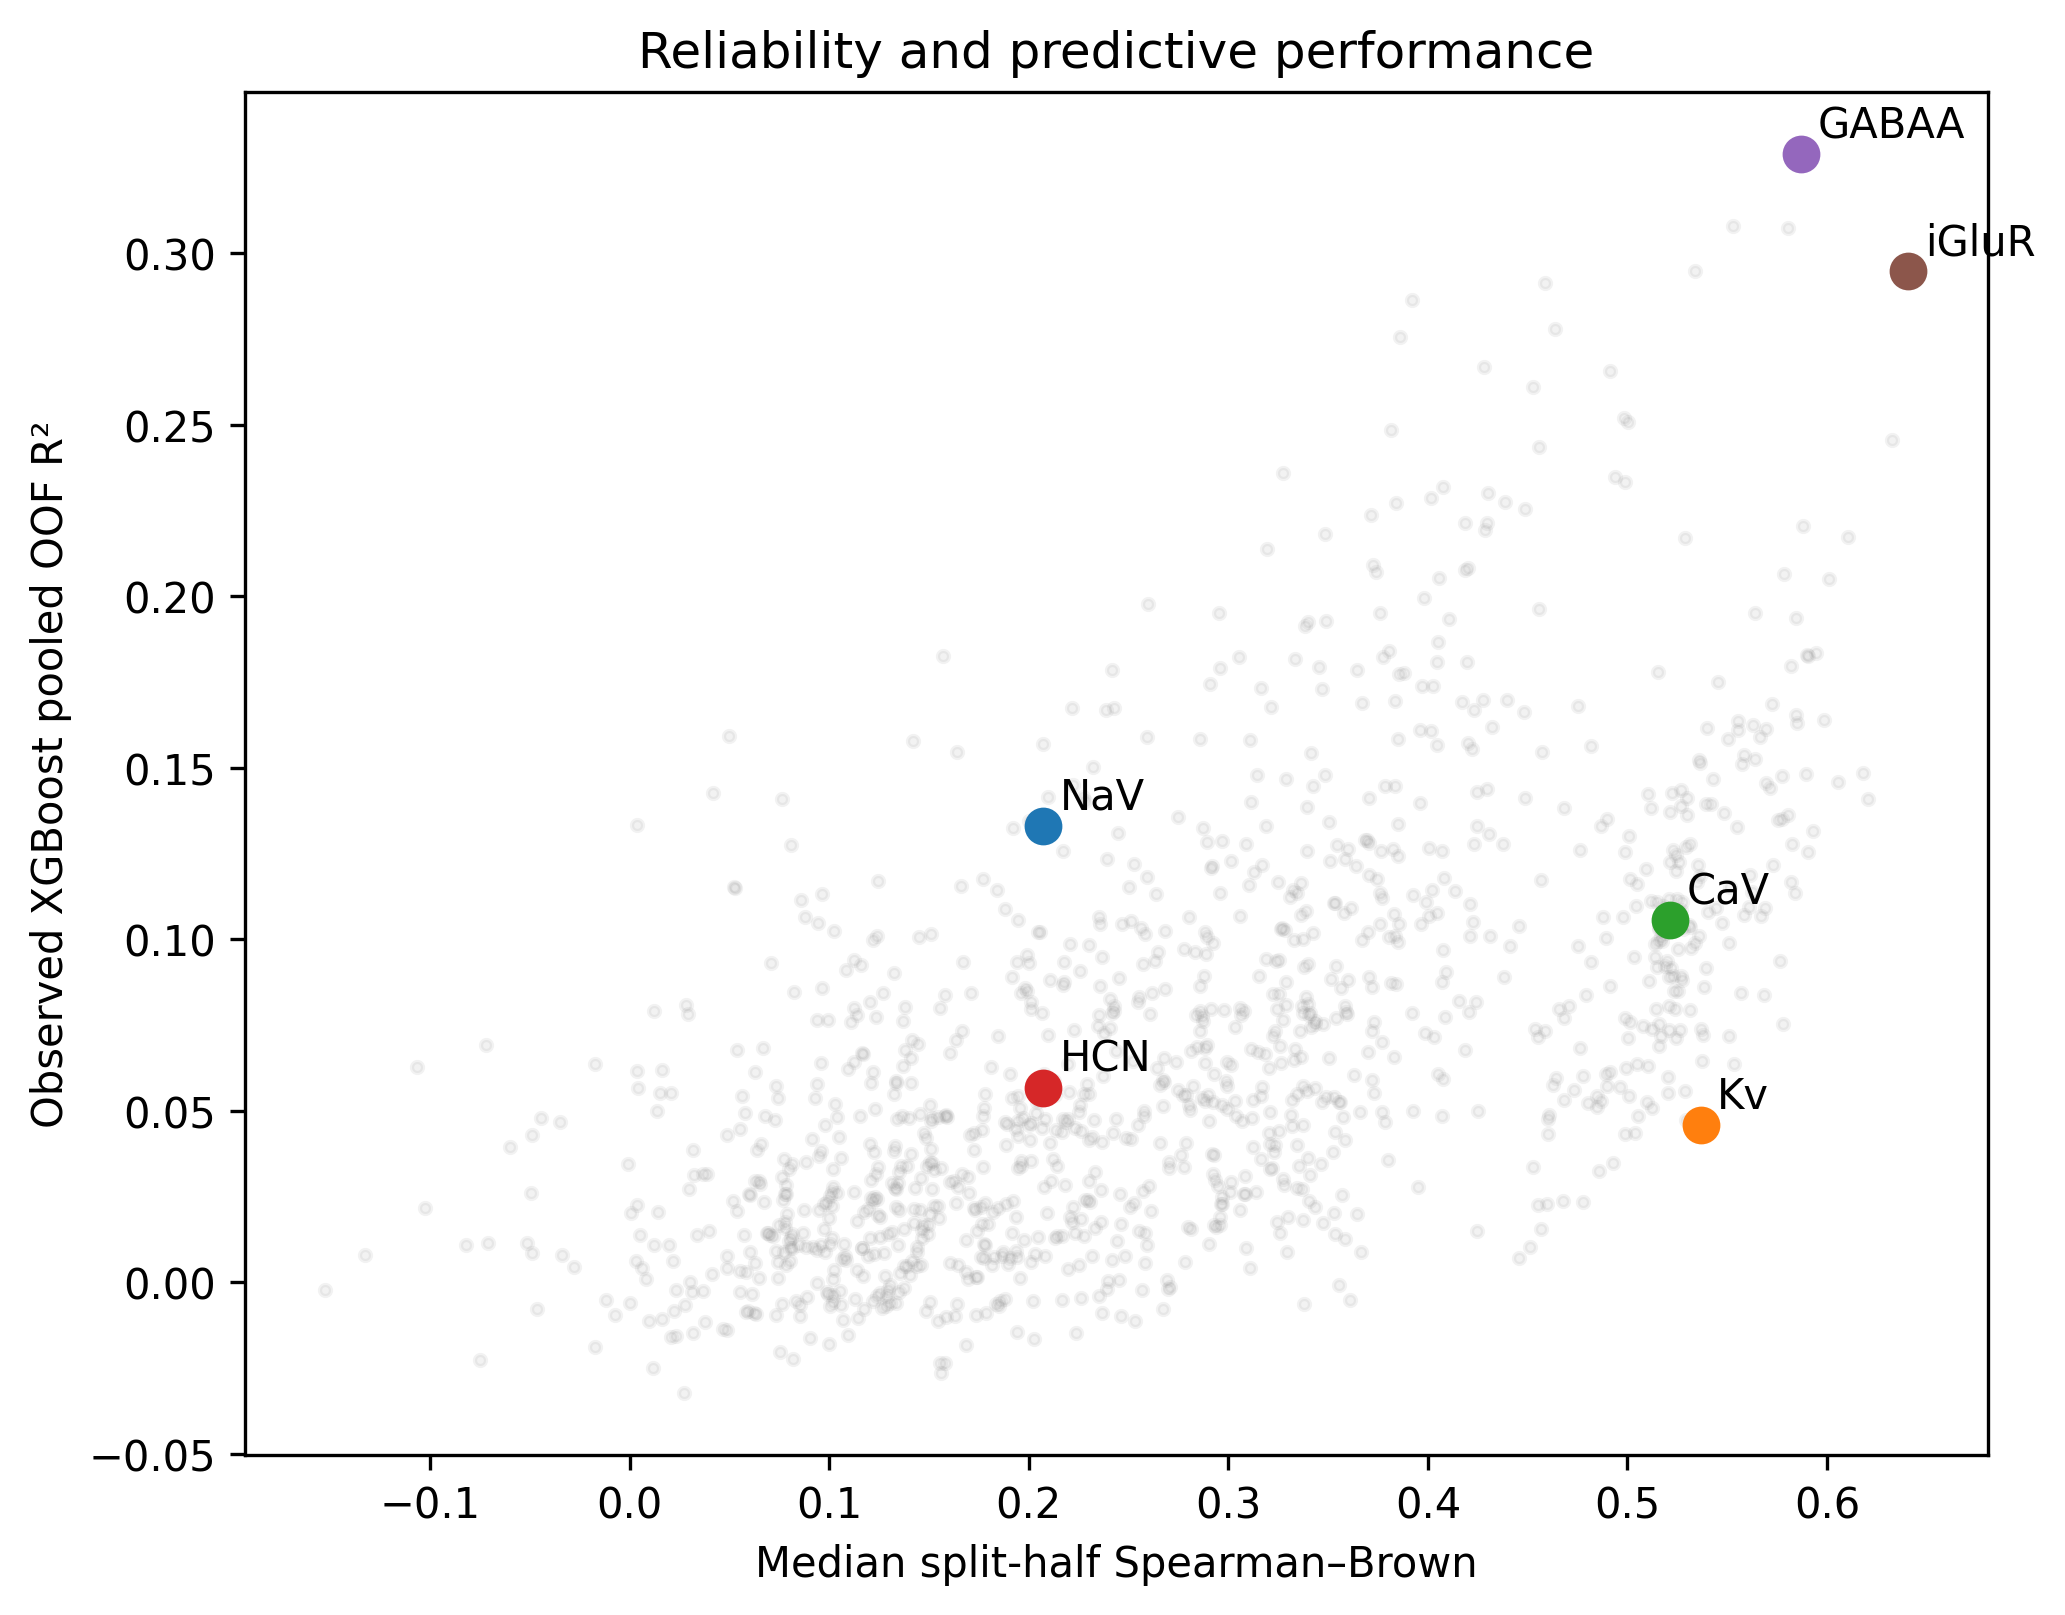
\includegraphics[width=.64\linewidth]{figures/Figure_S02_reliability_context.png}
\caption{Observed module consistency in the context of matched-control consistency. SB denotes Spearman--Brown correction.}
\label{fig:reliability}
\end{figure}

\section{NaV and Gene-Composition Sensitivities}
NaV6 is the prespecified primary target with 6 observed genes. NaV7 is a distinct 7-gene sensitivity using the exact release symbol \texttt{Scn2a1}; it does not replace missing \texttt{Scn2a} and is outside the primary matched-control BH family. Tables S29--S31 give the complete NaV6/NaV7 definitions and model metrics. Target-definition (Tables S32--S33) and leave-one-gene-out (LOGO; Table S34) results are available only under the 24-feature reference specification; no 23-feature refit was performed. Figure~\ref{fig:nav} summarizes the NaV comparison.

\sourcecaption{Prespecified NaV6 target and separate NaV7 sensitivity (Table S29).}
\begin{center}\tablefont
\begin{tabular}{lrrrrrrl}
\toprule
Target & Genes & $R^2$ & Pct. & $p$ & BH $q$ & Median SB & Role \\
\midrule
NaV6 & 6 & .133 & 95.1 & .0500 & .0999 & .207 & primary \\
NaV7 (+Scn2a1) & 7 & .078 & 79.1 & .2098 & -- & .274 & separate sensitivity \\
\bottomrule
\end{tabular}
\end{center}

\sourcecaption{Target-definition sensitivity under the 24-feature reference specification (Table S33; XGBoost).}
\begin{center}\tablefont
\begin{tabular}{lrrrrrl}
\toprule
Module & Mean $R^2$ & Std. mean $R^2$ & PC1 $R^2$ & Max $|\Delta R^2|$ & PC1 variance & Class \\
\midrule
NaV & .129 & .094 & .207 & .078 & .271 & moderately sensitive \\
Kv & .049 & .049 & .291 & .242 & .091 & composition-sensitive \\
CaV & .105 & .050 & .060 & .056 & .278 & moderately sensitive \\
HCN & .061 & .039 & .087 & .026 & .316 & robust \\
GABAA & .330 & .215 & .503 & .173 & .169 & composition-sensitive \\
iGluR & .294 & .186 & .221 & .108 & .279 & composition-sensitive \\
\bottomrule
\end{tabular}
\end{center}

\sourcecaption{Leave-one-gene-out sensitivity under the 24-feature reference specification (Table S34).}
{\tablefont
\begin{longtable}{@{}lllrrl@{}}
\toprule
Module & Omitted gene & Model & $R^2$ & $\Delta R^2$ & Classification \\
\midrule
\endfirsthead
\multicolumn{6}{l}{\small\itshape Table S34 continued}\\[2pt]
\toprule
Module & Omitted gene & Model & $R^2$ & $\Delta R^2$ & Classification \\
\midrule
\endhead
NaV & Scn3a & Dummy & -.002 & .001 & baseline reference \\
NaV & Scn3a & Elastic Net & .293 & .172 & stronger after omission \\
NaV & Scn3a & XGBoost & .307 & .178 & stronger after omission \\
NaV & Scn3a & Subclass Ridge & .278 & .177 & stronger after omission \\
NaV & Scn9a & Dummy & -.002 & .001 & baseline reference \\
NaV & Scn9a & Elastic Net & .013 & -.107 & weakened \\
NaV & Scn9a & XGBoost & -.010 & -.139 & weakened \\
NaV & Scn9a & Subclass Ridge & .007 & -.095 & weakened \\
HCN & Hcn2 & Dummy & -.001 & -.0003 & baseline reference \\
HCN & Hcn2 & Elastic Net & .034 & -.030 & mixed or partial \\
HCN & Hcn2 & XGBoost & .032 & -.028 & mixed or partial \\
HCN & Hcn2 & Subclass Ridge & .010 & -.031 & mixed or partial \\
HCN & Hcn3 & Dummy & -.001 & -.0001 & baseline reference \\
HCN & Hcn3 & Elastic Net & .123 & .059 & stronger after omission \\
HCN & Hcn3 & XGBoost & .131 & .071 & stronger after omission \\
HCN & Hcn3 & Subclass Ridge & .081 & .040 & mixed or partial \\
\bottomrule
\end{longtable}}

\section{Subclass Analyses}
The subclasses meeting the prespecified eligibility rule were Lamp5 (385 cells/171 donors), Pvalb (722 cells/302 donors), Sst (1,504 cells/393 donors), Vip (655 cells/248 donors). Within-subclass estimates are descriptive and unadjusted; they do not establish equivalence. Table S36 provides all four metrics. Table S35 asks the separate question of whether electrophysiology improves a Ridge model already given subclass labels; its intervals are unadjusted exploratory donor-cluster bootstrap intervals based on 5,000 draws.

\sourcecaption{Complete within-subclass $R^2$ grid (Table S36).}
\begin{center}\tablefont
\begin{tabular}{llrrrrrr}
\toprule
Subclass & Model & NaV & Kv & CaV & HCN & GABAA & iGluR \\
\midrule
Lamp5 & Elastic Net & .025 & -.022 & -.017 & .022 & -.076 & .018 \\
Lamp5 & XGBoost & -.054 & -.143 & -.288 & -.043 & -.157 & -.125 \\
Pvalb & Elastic Net & -.018 & .0005 & -.019 & -.034 & .042 & .019 \\
Pvalb & XGBoost & -.071 & -.047 & -.128 & -.114 & .017 & .029 \\
Sst & Elastic Net & .079 & .035 & .045 & .038 & .362 & -.020 \\
Sst & XGBoost & .074 & .039 & .015 & .001 & .334 & -.051 \\
Vip & Elastic Net & -.003 & -.009 & .002 & .001 & .019 & -.019 \\
Vip & XGBoost & -.044 & -.112 & -.091 & -.079 & -.0005 & -.015 \\
\bottomrule
\end{tabular}
\end{center}

\Needspace{14\baselineskip}
\sourcecaption{Electrophysiology increment beyond subclass-only Ridge (Table S35).}
\begin{center}\tablefont
\begin{tabular}{lrrrr}
\toprule
Module & Subclass Ridge & Ephys + subclass & $\Delta R^2$ & 95\% CI \\
\midrule
NaV & .102 & .136 & .034 & [.019, .049] \\
Kv & .042 & .065 & .023 & [.008, .037] \\
CaV & .104 & .114 & .010 & [-.002, .021] \\
HCN & .041 & .057 & .016 & [.002, .029] \\
GABAA & .177 & .319 & .142 & [.118, .166] \\
iGluR & .327 & .340 & .014 & [.003, .025] \\
\bottomrule
\end{tabular}
\end{center}

\begin{figure}[H]
\centering
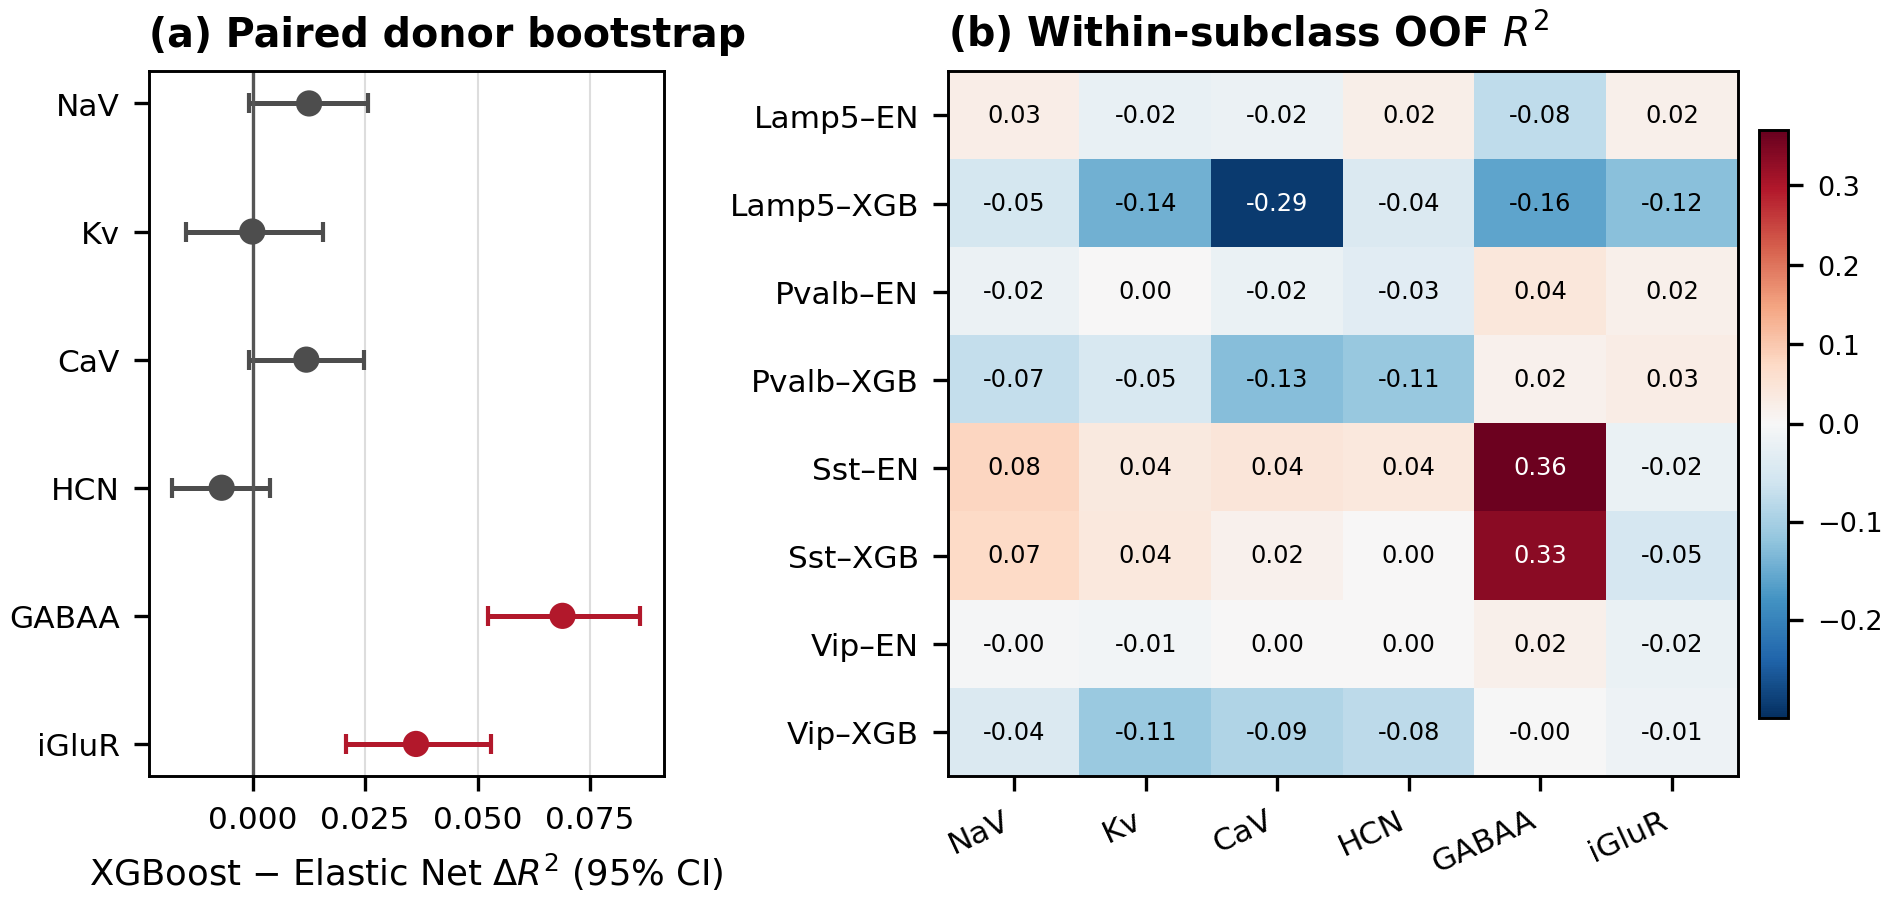
\includegraphics[width=.88\linewidth]{figures/Figure_S03_inference_and_subclass.png}
\caption{Formal model comparisons and within-subclass prediction. Subclass panels are descriptive and unadjusted.}
\label{fig:subclass}
\end{figure}

\section{Repeated Grouped CV and Calibration}
The 5 repeated donor-grouped splits characterize sensitivity to the split, not confidence intervals and not repeated-tuning uncertainty. Tables S37--S39 contain the complete repeated-CV metrics, calibration results, and top-decile enrichment results. The display below gives every model--module combination for repeated $R^2$ and calibration summaries.

\sourcecaption{Repeated donor-grouped CV, calibration, and top-decile enrichment (Tables S37--S39).}
{\tablefont
\setlength{\tabcolsep}{2.8pt}
\begin{longtable}{@{}llrrrrrr@{}}
\toprule
Module & Model & Repeat median & Repeat range & Primary & Slope & Pred./obs. SD & Top-decile ratio \\
\midrule
\endfirsthead
\multicolumn{8}{l}{\small\itshape Tables S37--S39 continued}\\[2pt]
\toprule
Module & Model & Repeat median & Repeat range & Primary & Slope & Pred./obs. SD & Top-decile ratio \\
\midrule
\endhead
NaV & Elastic Net & .134 & [.126, .137] & .121 & .963 & .361 & 1.140 \\
NaV & XGBoost & .140 & [.134, .144] & .133 & .910 & .403 & 1.155 \\
NaV & MLP & .092 & [.077, .101] & .082 & .668 & .495 & 1.156 \\
Kv & Elastic Net & .052 & [.044, .059] & .046 & .980 & .219 & 1.037 \\
Kv & XGBoost & .055 & [.050, .066] & .046 & .737 & .311 & 1.044 \\
Kv & MLP & .0003 & [-.015, .011] & -.015 & .465 & .467 & 1.044 \\
CaV & Elastic Net & .097 & [.083, .103] & .094 & .985 & .311 & 1.110 \\
CaV & XGBoost & .109 & [.101, .113] & .106 & .879 & .373 & 1.125 \\
CaV & MLP & .040 & [.029, .043] & .035 & .575 & .481 & 1.095 \\
HCN & Elastic Net & .061 & [.058, .066] & .064 & .927 & .273 & 1.122 \\
HCN & XGBoost & .046 & [.039, .052] & .057 & .790 & .313 & 1.126 \\
HCN & MLP & .013 & [.011, .017] & .011 & .533 & .402 & 1.122 \\
GABAA & Elastic Net & .259 & [.249, .263] & .260 & 1.005 & .507 & 1.149 \\
GABAA & XGBoost & .329 & [.328, .340] & .329 & 1.004 & .572 & 1.165 \\
GABAA & MLP & .314 & [.306, .316] & .314 & .860 & .661 & 1.156 \\
iGluR & Elastic Net & .258 & [.246, .262] & .258 & .996 & .510 & 1.109 \\
iGluR & XGBoost & .295 & [.284, .300] & .295 & .949 & .573 & 1.119 \\
iGluR & MLP & .214 & [.206, .222] & .206 & .744 & .651 & 1.101 \\
\bottomrule
\end{longtable}}

\section{Target Correlations}
Tables S40--S42 report Spearman correlations for raw, subclass-centered, and technical-adjusted targets. The strongest raw pair was CaV--iGluR ($\rho=.557$); GABAA--iGluR was weakly negative ($\rho=-.089$). Figure~\ref{fig:correlations} shows the raw matrix; the complete centered and adjusted matrices are provided in Tables S41--S42. Supported specificity is therefore not reducible to the strongest target correlation.

\begin{figure}[H]
\centering
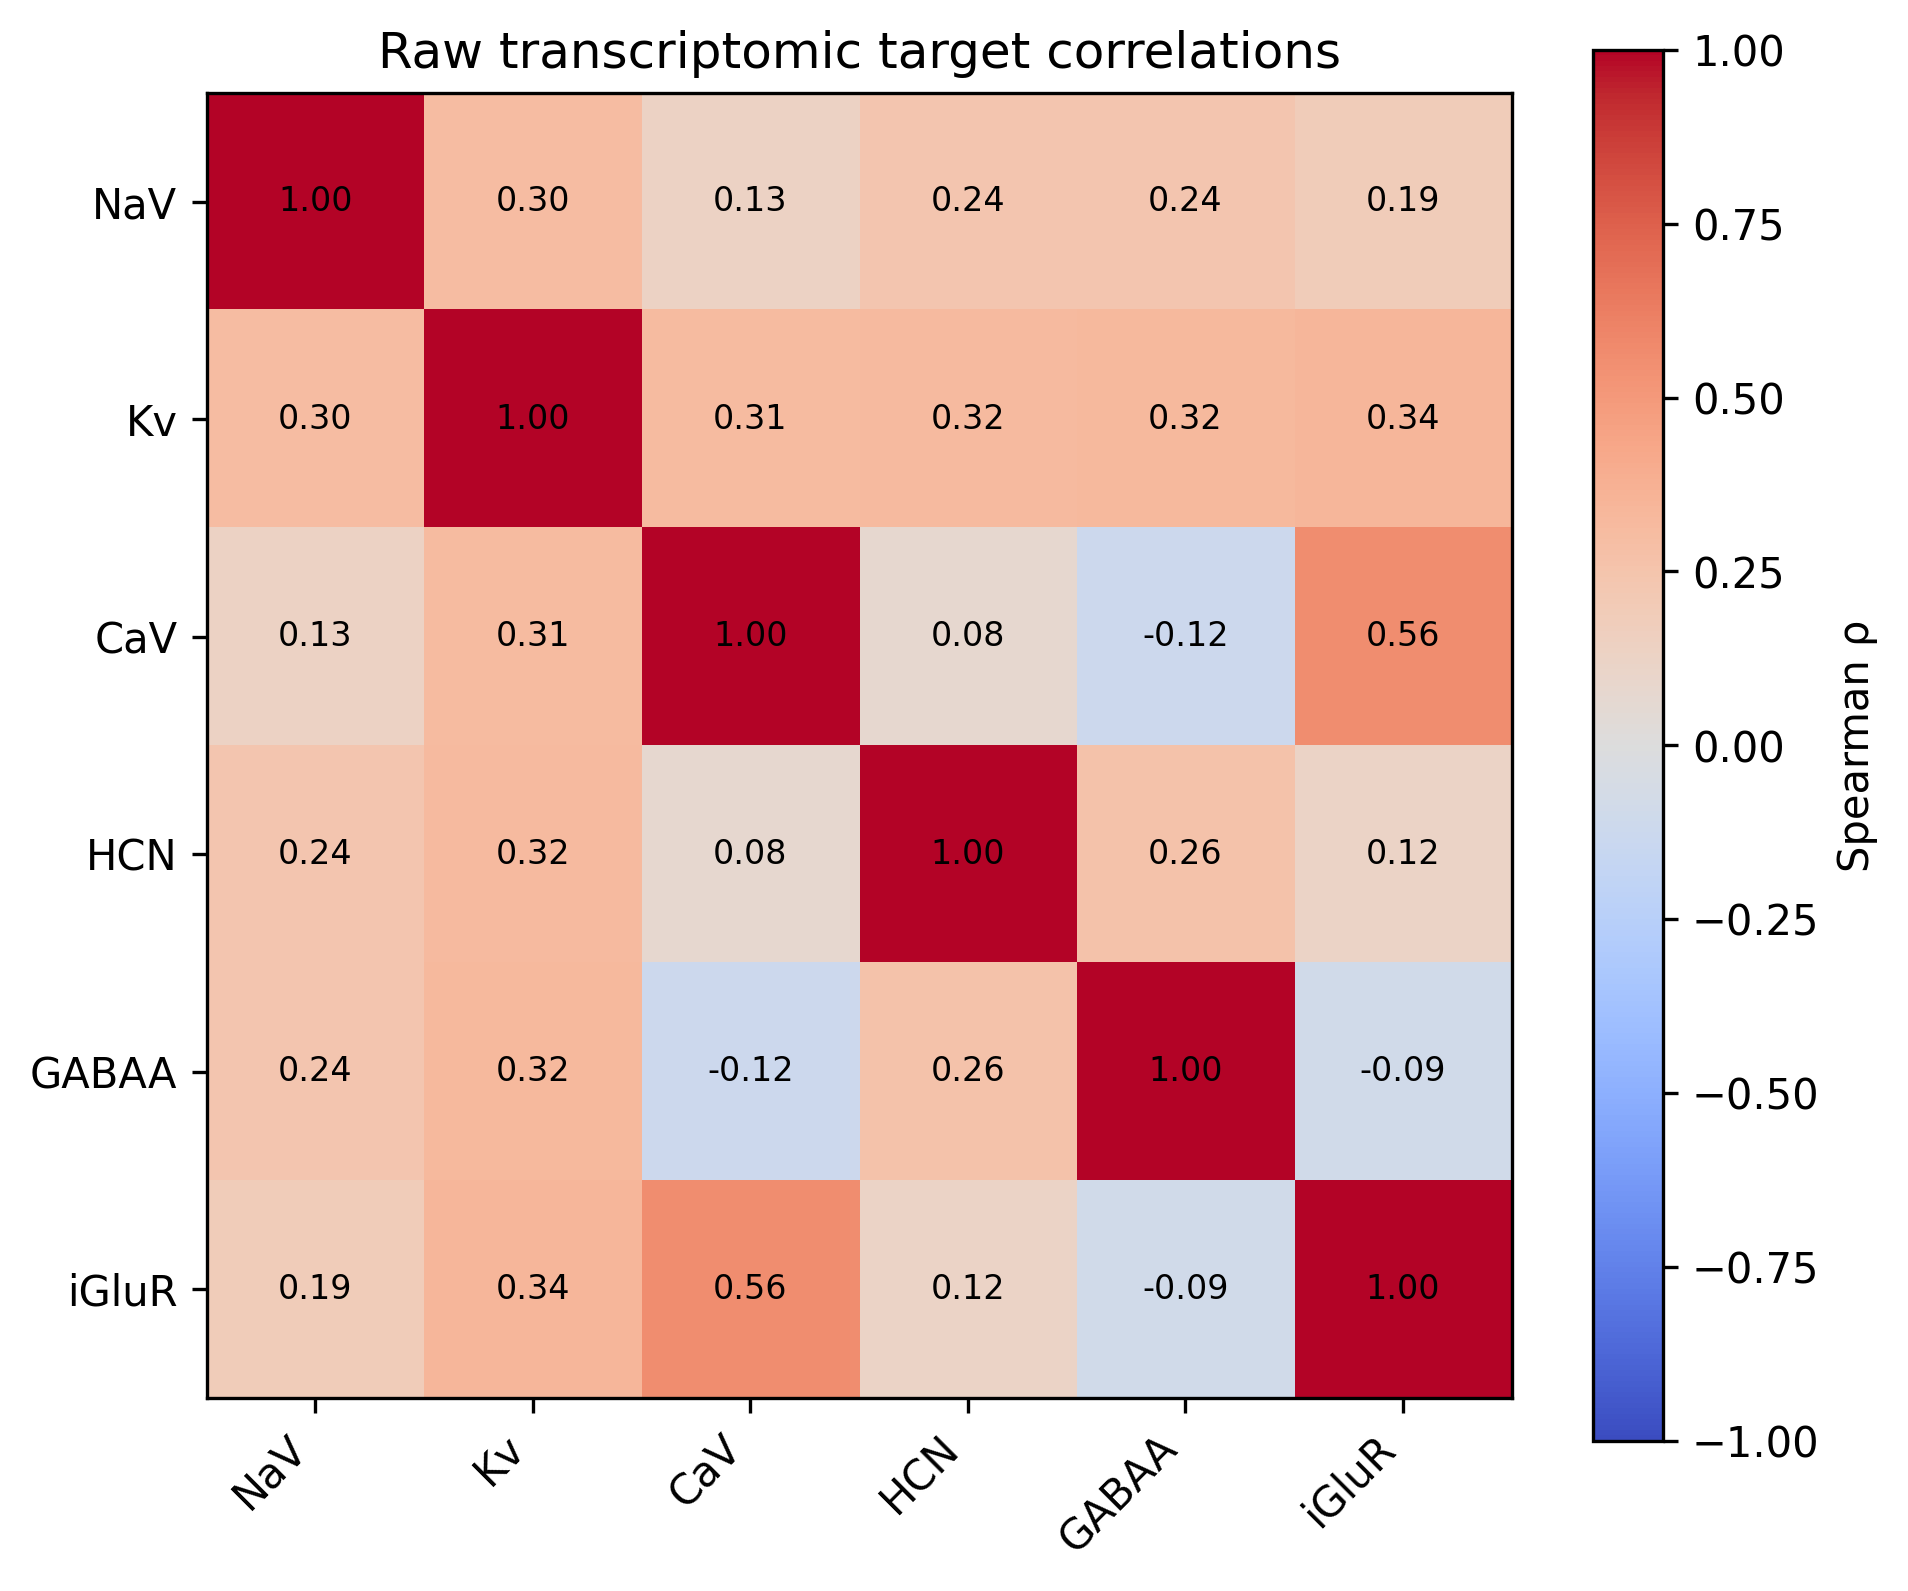
\includegraphics[width=.62\linewidth]{figures/Figure_S04_target_correlations.png}
\caption{Raw target-correlation matrix (Table S40). Complete subclass-centered and technical-adjusted matrices are reported in Tables S41--S42.}
\label{fig:correlations}
\end{figure}

\begin{figure}[H]
\centering
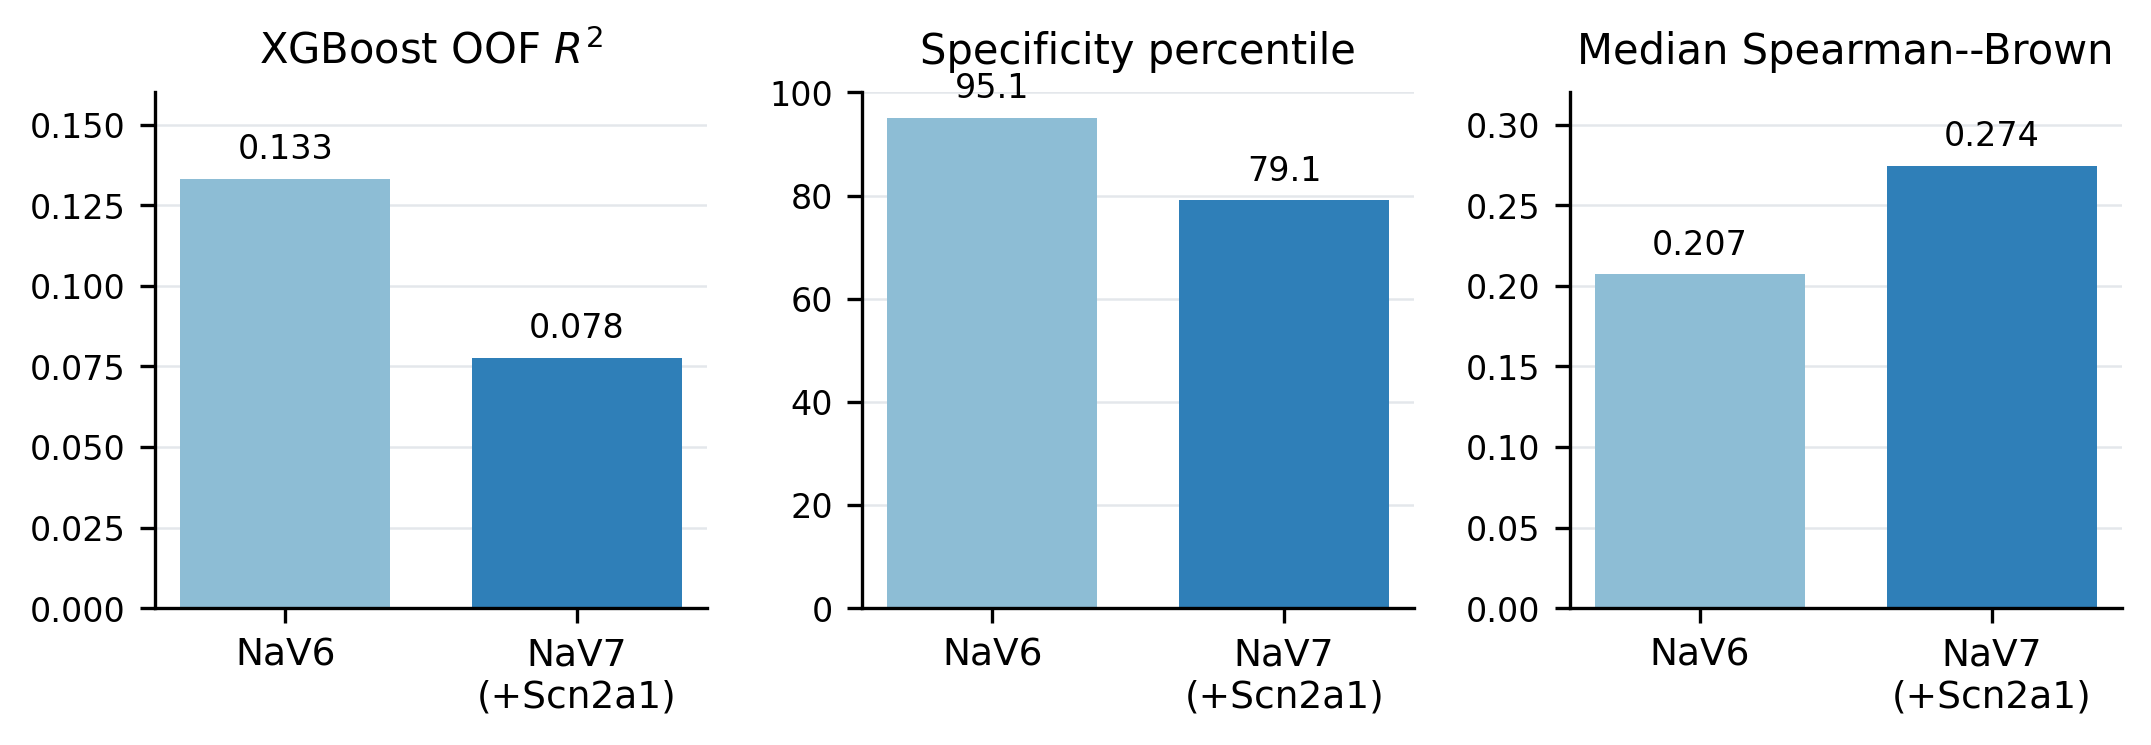
\includegraphics[width=.74\linewidth]{figures/Figure_S05_nav6_vs_nav7.png}
\caption{Comparison of the prespecified NaV6 target with the separate NaV7 sensitivity. Values are reported in Table S29. Adding exact \texttt{Scn2a1} increased split-half consistency but did not improve OOF prediction or matched-control specificity.}
\label{fig:nav}
\end{figure}

\section{Attribution and Correlated Predictors}
The 23 predictors were partitioned into 19 components at $|\rho|>.90$ (Table S43). Held-out TreeSHAP magnitudes were summed within components (Tables S44--S45) and compared with grouped absolute Elastic Net coefficients (Table S46). Because predictors are correlated, these summaries are predictive rather than causal and do not identify unique electrophysiological mechanisms.

\sourcecaption{Concordance between grouped TreeSHAP importance and grouped absolute Elastic Net coefficients (Table S47).}
\begin{center}\tablefont
\setlength{\tabcolsep}{2.7pt}
\begin{tabularx}{\linewidth}{@{}lrrrrYY@{}}
\toprule
Module & Groups & Rank $\rho$ & Top-3 overlap & Jaccard & SHAP top 3 & Elastic Net top 3 \\
\midrule
NaV & 19 & .507 & 2 & .500 & C01|C06|C09 & C01|C06|C18 \\
Kv & 19 & .754 & 2 & .500 & C01|C14|C17 & C01|C09|C17 \\
CaV & 19 & .533 & 2 & .500 & C01|C09|C18 & C01|C02|C18 \\
HCN & 19 & .667 & 2 & .500 & C01|C06|C09 & C01|C02|C06 \\
GABAA & 19 & .856 & 1 & .200 & C06|C09|C18 & C01|C06|C08 \\
iGluR & 19 & .468 & 2 & .500 & C01|C09|C18 & C01|C09|C17 \\
\bottomrule
\end{tabularx}
\end{center}

{\small\textbf{Component key for top-three entries (Table S43).} C01 = AP downstroke and width (long/short square); C02 = long-square AP fast-trough voltage; C06 = long-square AP threshold voltage; C08 = long-square AP upstroke; C09 = AP upstroke/downstroke ratio (long/short square); C14 = rheobase; C17 = short-square current; C18 = membrane time constant.}

\section{Reproducibility and Provenance}
All values in this report come from validated artifacts. The accompanying archive contains Tables S1--S50, Figures S1--S5 as PDFs and 300-dpi PNGs, the data-provenance ledger, SHA-256 checksums, software versions, validation results, and reproduction commands. Table S50 links each reported output to its source artifact. The reproducibility package excludes raw Allen data, copyrighted articles, credentials, absolute local paths, and temporary files.

\textbf{Software environment (Table S48).} Python 3.12.3; numpy 2.2.6; pandas 2.2.2; scipy 1.13.0; scikit-learn 1.9.0; xgboost 3.4.0; shap 0.52.0; matplotlib 3.8.4; pyarrow 25.0.0; h5py 3.14.0; joblib 1.5.3; PyYAML 6.0.1; pytest 9.1.1.

{\small\textbf{Validation and test results (Table S49).} \textit{Specificity-control pipeline}: 42 passed in 8.41s; \textit{23-feature modeling pipeline}: 76 passed in 20.43s; \textit{1,000-control extension}: 83 passed in 62.04s (0:01:02); \textit{Curated release}: 107 files; models\_fitted=0. Complete evidence paths are supplied in the machine-readable table.}

\textbf{Interpretive boundary.} The results support predictive association and, for GABAA and iGluR in the primary family, specificity beyond expression/detection-matched gene sets. They do not measure receptor abundance, conductance, causal regulation, or a formal biological ceiling.

\end{document}
